\marginnote{Texte issu de \cite{oraux_x_ens_1}}

\begin{marginfigure}[5cm]
    \centering
    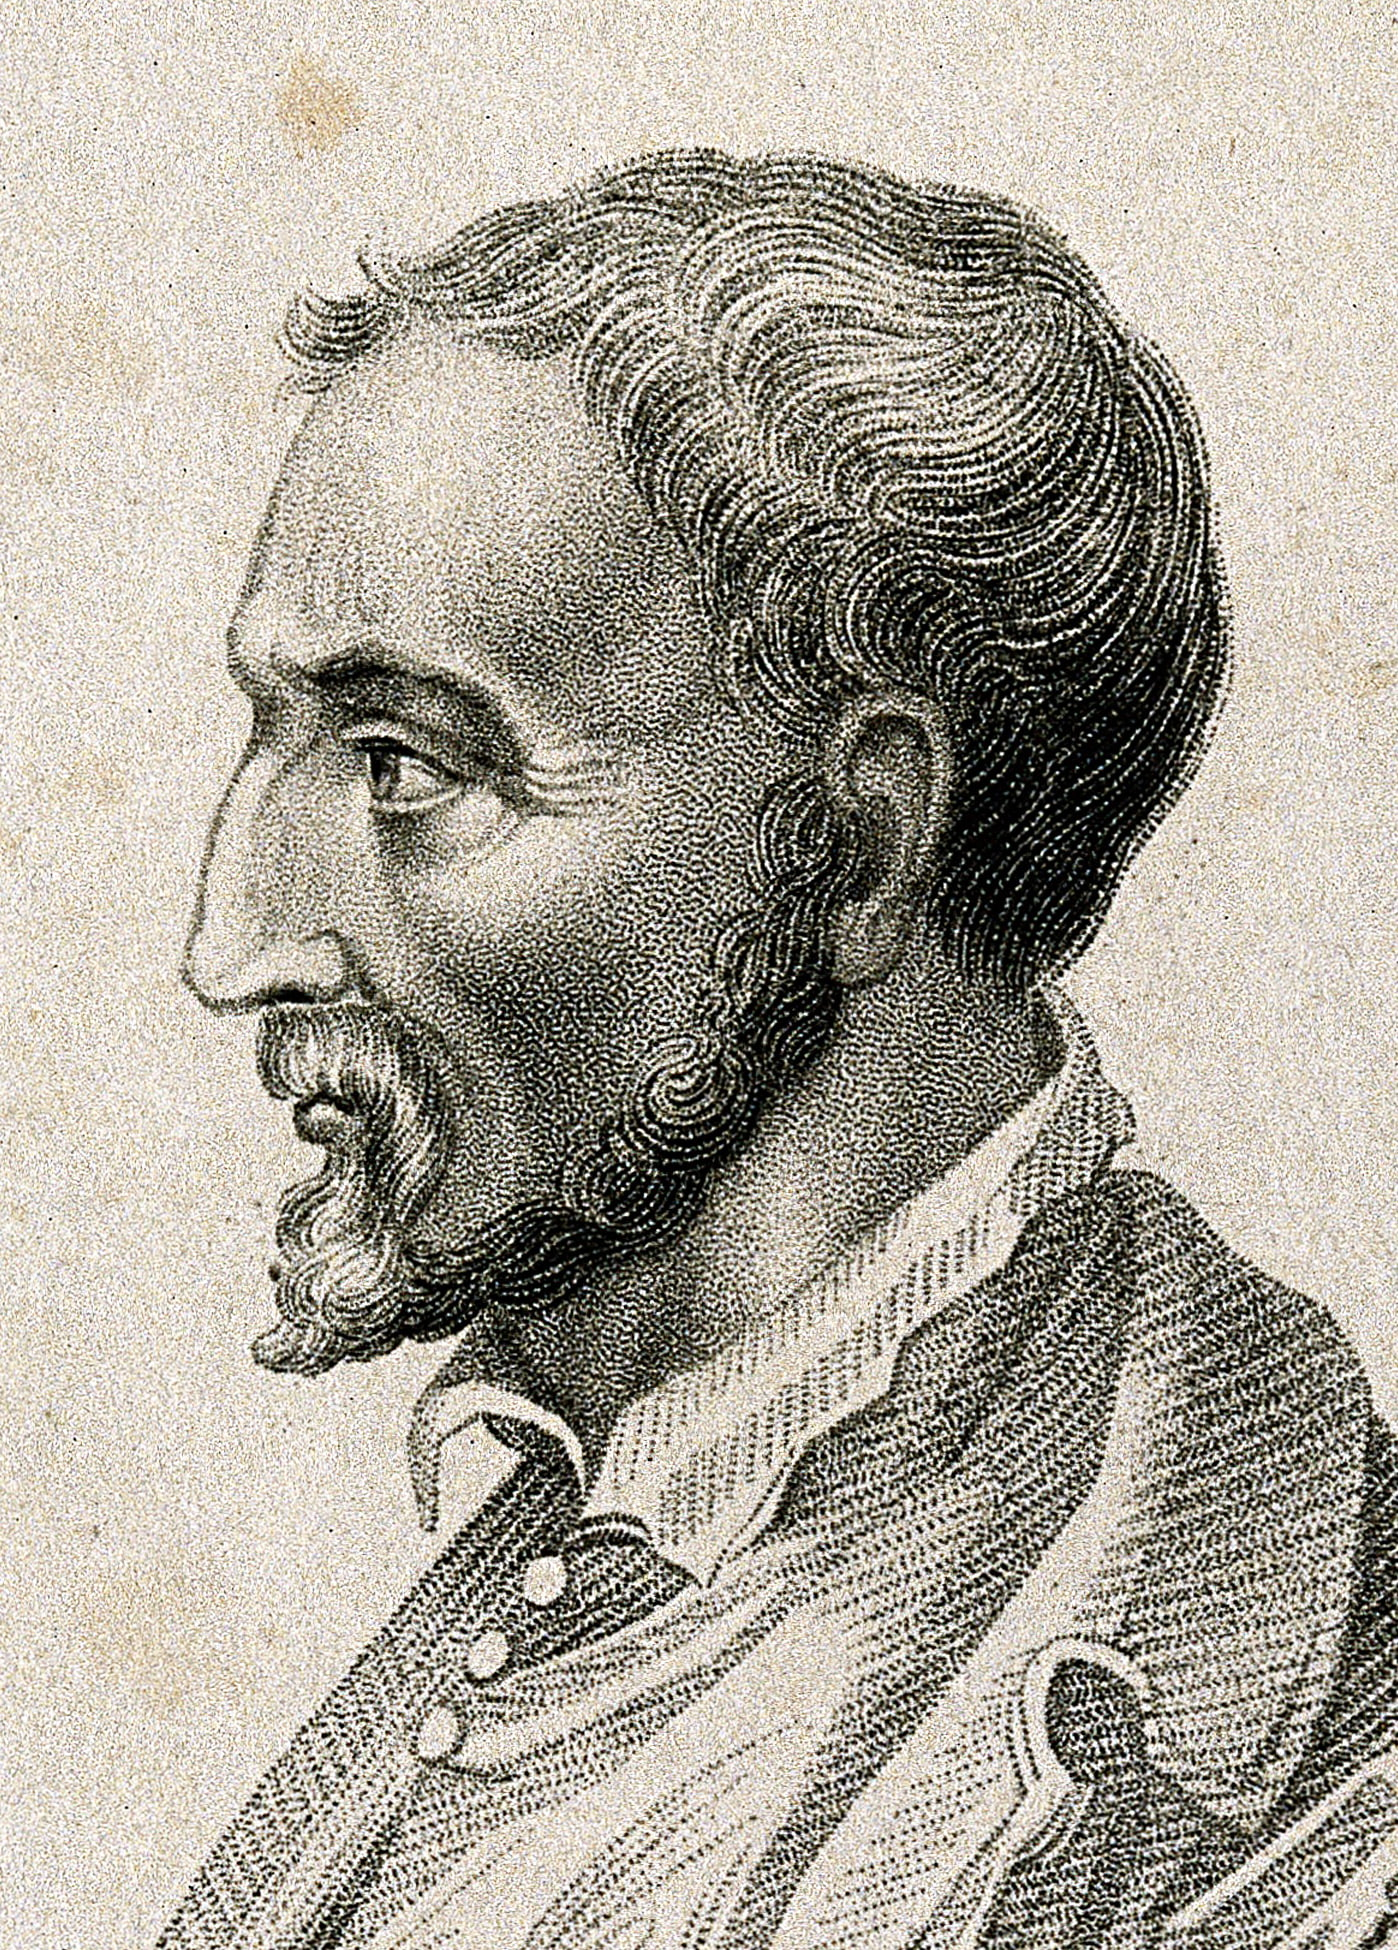
\includegraphics{images/jerome_cardan.jpg}
    \caption*{\centering Jérome \textsc{Cardan} (1501 - 1576)}
\end{marginfigure}

\textsl{
La théorie des équations polynomiales, qui précède de loin la définition formelle des polynômes, a été le propos essentiel de l'algèbre jusqu'au \textsc{xix}$^\me$ siècle. Elle est à l'origine de nombreuses notions: corps, nombres algébriques \dots Son développement est lié aux extensions successives de la notion de nombre: introduction des nombres négatifs, des nombres irrationnels, puis des nombres complexes. \\ 
Dès la plus haute Antiquité, on rencontre des exemples de résolutions d'équations. Les Babyloniens savent résoudre l'équation du second degré et les Grecs en font la base même de leur géométrie. \\
Après l'Antiquité, il faudra attendre le \textsc{xvi}$^\me$ siècle pour que des progrès substantiels apparaissent, dus à l'école italienne. \textsc{Scipone del Ferro}, \textsc{Tartaglia} et \textsc{Cardan} apportent la solution de l'équation du troisième dégré. L'équation générale est ramenée à la forme réduite $x^3 + px + q = 0$, dont une solution s'écrit
$$x = \sqrt[3]{-\frac{q}{2} + \sqrt{\frac{q^2}{4} + \frac{p^3}{27}}} + \sqrt[3]{-\frac{q}{2} - \sqrt{\frac{q^2}{4} + \frac{p^3}{27}}}.$$
Cette solution soulève des difficultés: si $\frac{q^2}{4} + \frac{p^3}{27}$ est négatif, cas où l'équation a des racines -- on le sait depuis \textsc{Archimède} -- on ne peut pas calculer $x$. Pour lever la difficulté, \textsc{Cardan} introduit timidement de nouveaux nombres, \say{ impossibles } ou \say{ imaginaires }. \textsc{Ferrari} et \textsc{Bombelli} résolvent l'équation du quatrième degré. \\
Grâce à l'école italienne, le théorie générale des équations algébriques se précise. L'équation étant mise sous le forme $P(x) = 0$, on prend conscience de l'importance du dégré de $P$ pour le nombre de solutions. On découvre que si $a$ est une racine de $P$, on peut factoriser par $x-a$. Les relations entre les coefficients et les fonctions symétriques des racines d'un polynôme apparaissent chez \textsc{Viète} (1540-1603), mais c'est \textsc{Girard} qui en 1629 leur donne toute leur extension. Suivi par \textsc{Newton}, il exprime les sommes des puissances des racines en fonction des coefficients. L'étude des fonctions symétriques des racines va se développer au \textsc{xvii}$^\me$ siècle avec \textsc{Waring} et au \textsc{xix}$^\me$ siècle avec \textsc{Cauchy}. \\
Au \textsc{xvii}$^\me$ siècle, la majorité des mathématiciens est convaincue qu'une équation de degré $n$ possède $n$ racines, celles-ci pouvant ne pas être réelles, mais il faut attendre \textsc{d'Alembert} pour trouver en 1724 une définition précise des nombres complexes (sous la forme $a + \sqrt{-1} b$). En 1799, \textsc{Gauss} fournit plusieurs preuves rigoureuses du \say{ théorème fondamental de l'algèbre } ou \say{ théorème de \textsc{d'Alembert}-\textsc{Gauss} }. \\
Des progrès sont réalisés également dans l'étude du nombre de racines réelles, et de leur signe. En 1637, \textsc{Descartes} énonce la règle qui porte son nom sur le nombre de racines positives d'un polynôme. On trouve dans \text{l'Algèbre} de \textsc{Rolle} (1690), la propriété suivante: entre deux solutions de l'équation $P(x)=0$, il existe au moins une solution de l'équation $P'(x)=0$. C'est \textsc{Sturm} qui formule, en 1829, les résultats les plus précis sur le nombre de racines réelles d'un polynôme. \\
Après les succès le l'école italienne au \textsc{xvi}$^\me$ siècle, les mathématiciens se sont attachés à trouver des formules analogues pour les dégrés suivants. Les réflexions sur cette question prennent un tour nouveau avec les travaux de \textsc{Lagrange} (1771), qui étudie les permutations des racines d'une équation laissant invariantes certaines fonctions de ces racines. Ces idées sont approfondies par \textsc{Cauchy} et \textsc{Ruffini}. \textsc{Abel} donne une démonstration rigoureuse de l'impossibilité de résoudre par radicaux l'équation générale de dégré $5$ en 1829. Enfin, en introduisant la notion de groupe, \textsc{Galois} énonce la condition générale à laquelle satisfait toute équation résoluble par radicaux (1831). \\
La distinction entre les nombres algébriques, racines d'un polynôme à coefficients entiers, et les autres qu'on nomme transcendants, date du \textsc{xvii}$^\me$ siècle, mais il faut attendre 1844 pour que \textsc{Liouville} démontre l'existence de nombres transcendants et plus longtemps encore pour que soit démontrée le trascendance de $\me$ (par \textsc{Hermite} en 1872) et celle de $\pi$ (par \textsc{Lindemann} en 1882). \\
Quant à la définition formelle des polynômes et à l'étude de leur structure, elles chemineront tout au long du \textsc{xix}$^\me$ siècle au rythme lent du processus d'axiomatisation de l'algèbre: par exemple, \textsc{Dedekind} introduit la notion de corps et définit les idéaux vers 1870.
}